\section{Introduction}

Nowadays data collection is omnipresent and the buzzword \textit{big data}\footnote{Big data is often described by the five V's: Volume, Variety, Velocity, Variability, Veracity \cite{Hilbert2015}} is referred to be the next "organizational challenge" that most of the industry is facing \cite{bigdata}. However, most of the research is done on the extraction of information from large datasets (so called Big Data Analysis). Therefore small datasets collected in day-to-day practice of professionals are often overlooked. 

Clinicians and hospitals collect a lot of data on their patients, the used therapies and the outcomes. Unfortunately this data is often not used to inform future practice. As a recent systematic review by \cite{survivalAnalysis} showed, the usage of statistical analysis has improved the survival analysis slowly. 

This project aims to implement an intelligent agent that provides advice based on statistical theory on the analysis of such data. The system depends on the design described in the related papers by Sassoon \textit{et al.} \cite{sassoon2014,sassoon2016,sassoon2016CD}. Especially the most recent publication will be used as solution to the problem of preferences over models in different context domains. 


This dissertation will first clarify the project aims and objectives in \autoref{sub:aims}. Second, the used methodologies are explained (see \autoref{sub:methodologies}). This is followed by a background research in \autoref{sec:background} providing a review of the theoretical aspects of argumentation frameworks and their extensions and the theory underlying statistical model selection. 
This will then be followed by a detailed project plan (see \autoref{sec:projectplan}) and the specification (see \autoref{sec:specification}). The consecutive chapters (see \autoref{sec:design} and \ref{sec:implementation}) are focusing on the actual implementation of the software as an \gls{RoR} web application. 
The report is concluded by a critical evaluation (see \autoref{sec:conclusion}) of the project and the delivered web application. 
The appendix contains the detailed description of the \glspl{use_case} (\autoref{app:use_cases}) that have been defined in \autoref{sec:design}, an installation guide to install the web application on a new machine (see \autoref{app:installation}).

\todo{Review at the end if structure still applies}

\subsection{Project Aims and Objectives} 
\label{sub:aims}

The aims of this project can be divided into a list or primary and secondary goals. For a successful project progression the following primary objectives have to be reached:
\begin{itemize}
	\item General explanation and summary of \glspl{AF}, \glspl{EAF}, statistical model selection and the definition of preferences between models related to \glspl{CD}.
	\item Development of an \gls{RoR} web application that implements the requirements proposed in \cite{sassoon2014,sassoon2016CD} including but not limited to:
	\begin{itemize}
		\item An approach to instantiate and solve \glspl{AF} and \glspl{EAF}.
		\item The ability to store, manage and reuse research questions, analysis, preferences for statistical models on different datasets.
		\item An easy to use user interface to upload data collected during clinical studies and run analyses in an interactive way using the theory proposed by Sassoon \textit{et al}.
		\item The ability to deal with preferences between models on a meta-level using \glspl{EAF} while taking into account global and personal (end user) preferences. The approach proposed in \cite{sassoon2016CD} involving \glspl{CD} will be used.
		\item A user rights management to allow the system to be used by clinicians, statisticians and super-users (admins).
		\item A small set of statistical models and their assumptions integrated in the system (provided by Sassoon in \cite{sassoon2016CD}).
		\item A comprehensive set of unit and integration tests of the system.
		\item Hosting of this web application at a public accessible provider.
	\end{itemize}	
	\item The system should provide the end user with an explanation why a statistical model should be used, and why one model might be preferred over another one.
\end{itemize}

\bigskip

The secondary goals are desired to be achieved but do not influence the successful finalisation of the project. These objectives are the following:
\begin{itemize}
	\item A documentation of the developed system providing information on how to use it and an overview over the key components of the application.
	\item A reusable implementation to solve standard \glspl{AF} in Ruby as a \texttt{gem} including documentation and a comprehensive set of unit tests.
	\item A reusable implementation to solve \glspl{EAF} in Ruby as a \texttt{gem} including documentation and a comprehensive set of unit tests.
	\item Extended sets of statistical models and their assumptions.
	\item A graphical representation of the arguments explaining the actual analysis outcome of the system.
\end{itemize}


\subsection{Methodologies of the Project}
\label{sub:methodologies}
This project will be developed in an agile way. To ensure that it meets the requirements described by Sassoon \textit{et al.} (\cite{sassoon2014, sassoon2016, sassoon2016CD}, see \autoref{sub:statistical_model_selection}), the main author of that paper is treated as a client or \gls{product owner} during the requirements analysis and the testing phase. For the actual development process the Use-Case 2.0 approach by Jacobson \textit{et al.} \cite{jacobson2011usecase} is used as it provides a great way to communicate, specify and iterate over functional (independent) parts of the system with non-developers. Due to its descriptive nature it does not require any knowledge about the actual process to be easy understandable. However, this methodology will be explained and introduced in detail later in this dissertation (see \autoref{sec:design}). 

As a project communication and management tool Trello\footnote{\href{http://www.trello.com}{www.trello.com}} is utilised as it provides an easy-to-use and interactive way of dealing with cards (in our case use-cases and tasks) and to group them. During the project planning it has been decided to break down the development into  four release cycles (RC~1 - 4, see \autoref{sec:projectplan}), as this will provide a modularisation of the project and allows early feedback on it. However track of the already achieved intermediate steps and the actual progress of the development process can be recorded efficiently with Trello. Labels and different lists visualise the status and progress of each task and use-case (see \autoref{fig:trello}).


\begin{figure}[h]
\centering
	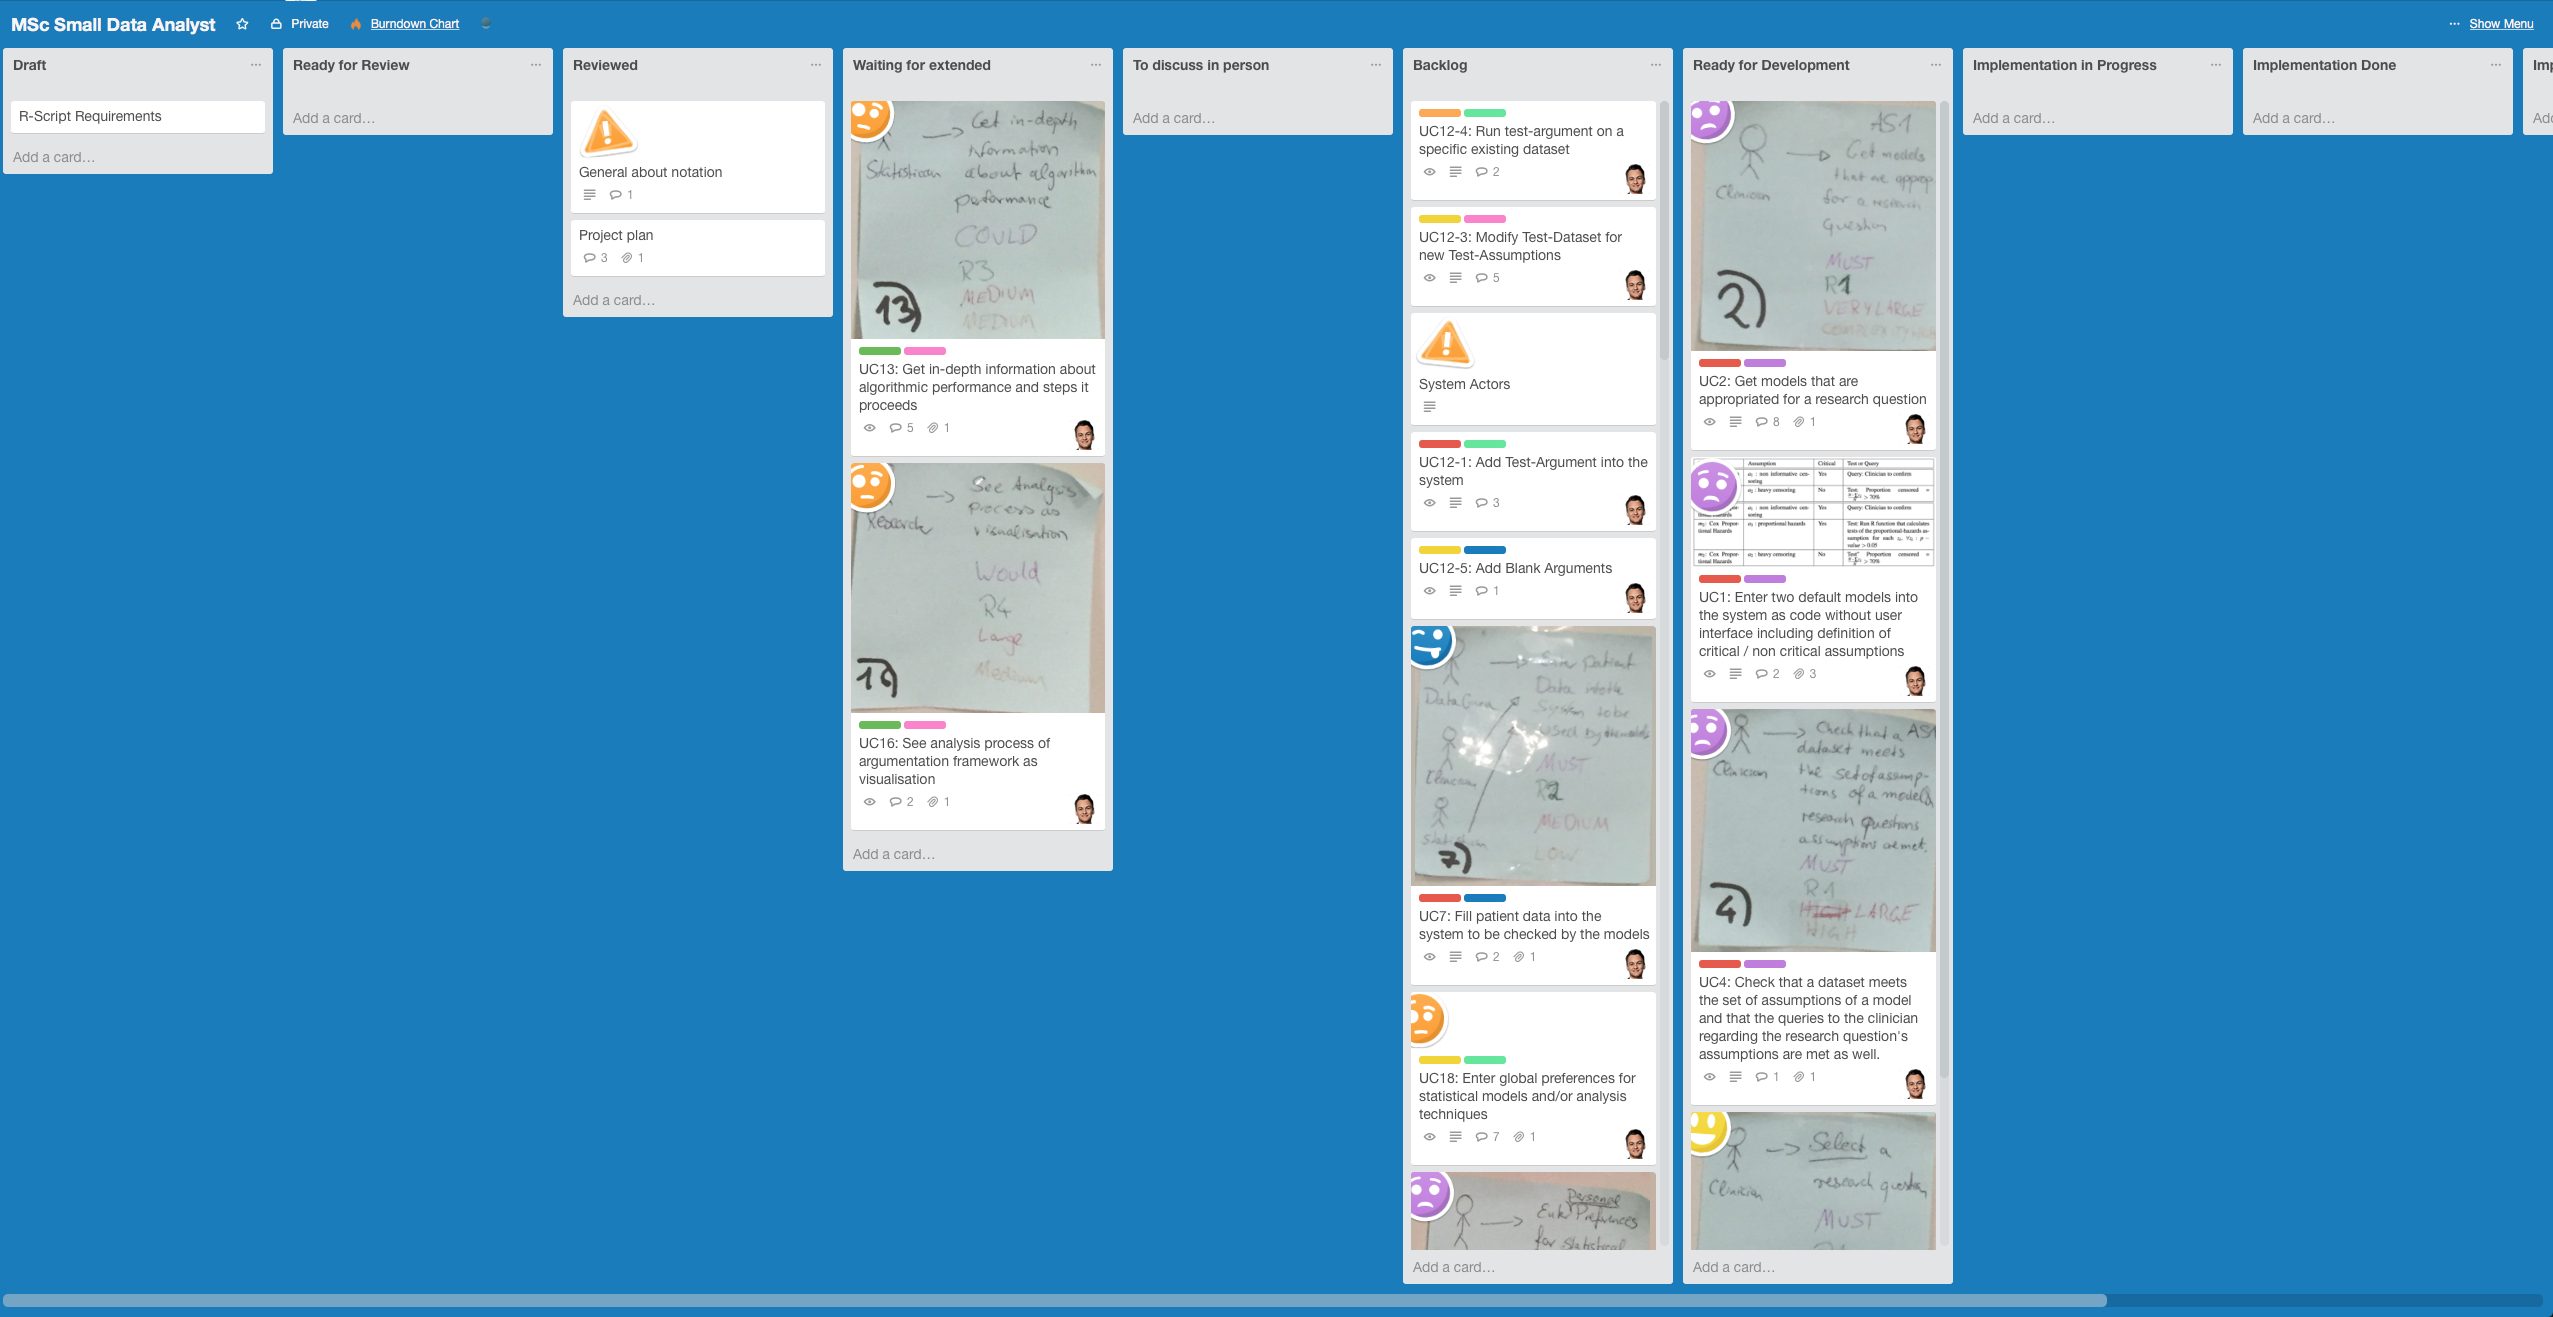
\includegraphics[page=1,width=\textwidth]{figures/trello}
\caption{Screenshot of the used Trello board used as project management tool}
\label{fig:trello}
\end{figure}

\subsection{Supplementary Resources}

During this Masters Project a web-application has been developed which is public available on \href{http://small-data-analyst.herokuapp.com}{http://small-data-analyst.herokuapp.com}. Users can sign-up (needs approval of an administrator, please reach out to the author if you have any questions related to that) and upload there own datasets. Some of the existing research questions are publicly available and shared between all users of the application. However -- if required -- the source code is available on \href{https://github.com/sebastianzillessen/small-data-analyst}{Github}\footnote{\href{https://github.com/sebastianzillessen/small-data-analyst}{https://github.com/sebastianzillessen/small-data-analyst}} and a installation instruction can be found in the appendix \autoref{app:installation}. A detailed list of used third-party applications can be found in \autoref{app:3rdparty}.

